\section{Overview}
In this section, we introduce the data model, discuss the problem, and finally, present a brief overview of existing solutions as well as our approach.

%\subsection{Data} We focus on heterogeneous Web data  RDF and other types of data that can be modelled as graphs. Closely resembling the RDF data model, we employ a graph-structured data model where every dataset is conceived as a graph $G \in\mathbb{G}$ comprising a set of triples: 

\subsection{Data} 

We focus on RDF data and other types of data that can be modelled as graphs. Closely resembling the RDF data model, we employ a graph-structured data model where every dataset is conceived as a graph $G \in\mathbb{G}$ comprising a set of triples: 

\begin{definition}[Data Model] A dataset set is a graph $G$ formed by a set of triples of the form $(s, p, o)$ where $s \in U$ (called subject), $p \in U$ (predicate) and $o \in U \cup L$ (object). Here, $U$ denotes the set of Uniform Resource Identifiers (URIs) and $L$ the set of literals. Every literal $l \in L$ is a bag of tokens, $l = \{t_1,\ldots,t_i,\ldots,t_n\}$, drawn from the vocabulary $V$, i.e. $t_i \in V$.  
\end{definition} 

With respect to this model, \emph{instances} are resources that appear at the subject position of triples. An instance representation can be obtained from the data graph as follows:

\begin{definition}[Instance Representation] The instance representation $IR: U \times \mathbb{G} \rightarrow \mathbb{G}$ is a function, which given an instance $s \in U$ and a graph $G \in \mathbb{G}$, maps $s$ to a set of triples in which $s$ appears as the subject, i.e. $IR(s) = \{ (s, p, o) | (s, p, o) \in G, o \in L \}$. 
\end{definition} 

Thus, an instance is basically represented through a set of \emph{predicate-value} pairs, where values are bags of tokens. \todo{add a graph to provide example, also, provide one example for instance representation} 
We will use the terms instance and instance representation interchangeably from now on. Note that for the sake of presentation, only the outgoing edges $(s, p, o)$ of an instance $s$ are considered while incoming edges (triples where $s$ appears as the object) can also be added to the representation of $s$. 

\subsection{Problem - Find Instance Matches and Match Candidates} \emph{Instance matching} is about finding instances that refer to the same real-world object based on their representations extracted from the data. In this paper, we tackle the problem of \emph{instance matching across multiple datasets}: given instances of a \emph{source dataset} $G_s$, the problem is to find instances in others datasets, collectively referred to as the \emph{target dataset} $G_t$, which represents the same real world object. 

\textbf{Challenges.} Compared to the single dataset setting, this problem entails additional challenges especially when the data is heterogeneous not only at the data but also schema level. In this regard, \emph{data-level heterogeneity} means that for the same property, instances referring to the same object may have different values, or different syntactical representations of the same value. \todo{For instance, the values "Michael Jackson" or "Jackson, Michael" can be both used as the value of the property name of an instance representing  Michael Jackson.} (1) \emph{Schema-level heterogeneity} arises when there is only little or no schema overlaps between the datasets. That is, instances referring to the same object may be represented by different predicates, or different representations of the same predicates. Finding different representations of the same predicate is part of a problem also known as schema matching. Another challenge in this multiple dataset setting is (2) \emph{efficiency}: for instance matching, a scheme is needed to determine how to compare two given instances; we will show that especially with schema heterogeneity, finding the best scheme for matching across heterogeneous datasets involves a greater search space and more feedback information (training data). Searching through all possible solutions and obtaining feedback information to evaluate them is expensive especially when we consider the online learning of instance matching schemes that requires access to data from remote endpoints. \todo{discuss in intro that we need schemes for individual instances, and motivates and explain the concept of online learning of instance schemes: involves live access to remote endpoints that host fresh version of the datasets.}

\textbf{Computing Instance Matches.} More precisely, an \emph{instance matching scheme} is a (weighted) combination of similarity function predicates, $\sum_i{w_i \sim(p_i)} > \alpha$.  Every $\sim(p_i)$ is a function, which given two instances $s_i$ and $s_j$, returns the similarity between these instances based on their similarity on the values of the predicate $p_i$. The scheme computes the overall similarity between $s_i$ and $s_j$ by combining the similarities obtain for individual predicates and determines them as a \emph{match} when its exceeds the threshold $\alpha$. Clearly, such a scheme focus on data-level heterogeneity. Given $s_i$ and $s_j$ are in the source and target datasets, respectively, and these datasets vary in schema, an extended scheme of the form $\sum_i{w_i \sim(\langle p^s_m,p^t_n \rangle_i )} > \alpha$ is needed to capture that the values of the source predicate $p^s_m$ shall be compared with values of the target predicate $p^t_n$. In other words, when the predicates in the source and target are not the same, comparable pairs of predicates have to be found and incorporated into the scheme. 
%The similarity of $s_i$ and $s_j$ is computed by combining the similarity values obtained for all individual pairs of comparable predicates captured by the scheme. They are considered as a \emph{match} when it .
In fact, this problem entails the subproblems of (A) finding the pair of comparable predicates $\langle p^s_m, p^t_n \rangle$ (schema matching) as well as (B) choosing and (C) weighting them, and determining the (D) similarity functions $\sim$ (e.g. Jaccard distance) and (E) thresholds $\alpha$.  

\textbf{Computing Instance Match Candidates.} Instead of solving all these problems, some instance matching solutions focus on the blocking step, which aims to quickly select candidates matches (hence also referred to as the \emph{candidate selection} step). Instead of using a combination of similarity function predicates, candidate selection simply employs a (conjunction of) blocking key(s), i.e. $\bigwedge \sim(\langle p^s_m,p^t_n \rangle_i)$ (called \emph{candidate selection scheme}), where $\sim$ is a binary function that returns whether the two values of $p^s_m$ and $p^t_n$ match or not. Here, the predicates $p^s_m$ and $p^t_n$ constitute the pair of comparable blocking keys while their values are called \emph{blocking key values} (BKV). Usually, the similarity function is based on exact value matching or value overlap. That is, two instances form a \emph{candidate match} if their blocking key values are the same or overlap on some tokens. 
Mostly, $\sim$ is defined manually such that candidate selection amounts to the problem of (A) finding comparable predicate pairs and (B) choosing the most selective ones as blocking key pairs. 
%Fig. 1 depicts the whole instance matching process described here. This paper focus on the candidate selection part of the problem.
Often, candidate selection is performed as a preprocessing step, producing results that are further refined by a more effective instance matcher that also tunes the weights and threshold to obtain better results. 


%\begin{figure} [ht]
% 
%\centering
%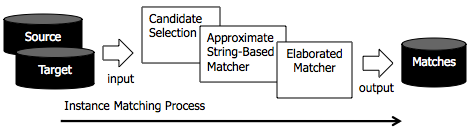
\includegraphics[scale=0.5]{p1.png}
%\caption{Instance matching process overview.} 
%\vspace{-2pt}
%\label{fig:space}
%\end{figure}

 

\subsection{Existing Solutions} 
State-of-the-art matching systems are based on supervised learning, leveraging training data as feedbacks to evaluate candidate schemes~\cite{DBLP:conf/vldb/ChaudhuriCGK07}. Basically, optimal schemes found are those which maximize the coverage of positive examples while avoiding negative examples. They are geared towards homogeneous datasets, focusing on the learning of schemes of the type $\sum_i{w_i \sim(p_i)} > \alpha$ as discussed above. It has been shown that in fact, the underlying learning strategies can also be used to obtain the extended schemes $\sum_i{w_i \sim(\langle p^s_m,p^t_n \rangle_i )} > \alpha$. Instead of all combinations of individual predicates, the search space would have to include all combinations of all possible pairs of predicates. 

Since obtaining representative training data across datasets is difficult, recent approaches that specifically target heterogeneous data derive schemes directly from the data. However, unsupervised approaches of this kind focus on the more simpler problem, namely the learning of the candidate selection schemes $\bigwedge \sim(\langle p^s_m,p^t_n \rangle_i)$. For instance, Song and Heflin~\cite{DBLP:conf/semweb/SongH11} assume precomputed schema mappings such that the comparable predicate pairs are known. They propose to choose them based on their coverage and discriminability; two metrics derived from the data basically reflecting the number of instances a given predicate can be applied to and how well it distinguishes them. Based on manually defined coverage and discriminability threshold, the best pairs of comparable blocking keys are selected. 
%Instances are then indexed by their BKVs and candidate sets are formed by searching on the index for overlapping tokens. This candidate selection is combined with another matcher, which further applies approximate string matching on the BKVs of the remaining candidates and filter those that are below a given threshold. 
%In this step, both the similarity function and the threshold are manually defined. Finally, the candidates sets generated are delegated to an arbitrary more elaborated matcher that finds the exact matches. 

As an alternative, a schema-agnostic approach~\cite{DBLP:conf/wsdm/PapadakisINF11} has been proposed for candidate selection. It does not use predicates for matching but treat instances simply as bags of value tokens. Instances form matches when they have some value tokens in common. Therefore, instances which share the same token (in any predicate) are placed in one candidate set. This approach does not require any effort for learning the scheme and is particularly suited when there is a lack of schema overlap such that only few or no comparable predicates exist. The problem with this is that the candidate sets produced are highly redundant because instances are often placed in multiple candidate sets. Consequently, this work employs much more additional processing to further refine these candidate sets. 


\subsection{Existing Solutions vs. Our Solution}
In this work, we tackle the problem of instance matching. However, we focus on the problem of learning the candidate selection scheme and simply use the resulting scheme in combination with an existing matcher to refine candidate results. 

It has been shown that the use of schema knowledge improves precision but considerably decreases the coverage of correct matches~\cite{DBLP:conf/wsdm/PapadakisINF11} (recall). In this work, we propose a supervised learning strategy to incorporate predicate information into the candidate selection scheme that considerably improves both measures compared to this previous work~\cite{}. \todo{what have to be cited here? what previous work do you mean?}

The main difference between this and both the existing supervised and unsupervised learning strategies lies in the granularity of the learned scheme. Instead of using one scheme for all instances, our solution may yield different schemes for different source instances. This separate treatment of instances is introduced to specifically deal with the heterogeneity problem: for instance, two distinct drugs on Sider dataset, named Alpraxolan and Morphine, have two different schemes for mapping to the same drugs on Drugbank Dataset. Alpraxolan uses the scheme $\langle \verb+sider:label+,\verb+drugbank:drugname+ \rangle$, while Morphine uses the scheme $\langle \verb+sider:name+, \verb+drugbank:synomym+ \rangle$,  Using these more fine-grained schemes, we show that the quality of results produced by our approach is superior than those produced by existing supervised~\cite{DBLP:conf/vldb/ChaudhuriCGK07} and unsupervised approaches~\cite{DBLP:conf/semweb/SongH11}. 

Another aspect that has been neglected so far is time efficiency. More precisely, works on finding the scheme as discussed above focus on the quality of matches. On the other hand, there are works on executing similarity joins and building blocking indexes, focusing on how to process the schemes efficiently. In other words, more emphasis is put on the efficiency of execution and less on the efficiency of learning the scheme. The efficiency of learning became crucial when data is accessed over remote endpoints, where minimize the data access is necessary to be make any solution feasible.  

Further, how well a scheme can be optimized for time efficiency depends on the nature of the scheme itself. Some schemes are inherently expensive, requiring a large amount of data to be loaded and to be joined. Further, schemes that produce the same result quality may vary in terms of runtime efficiency. Thus, optimized execution performance cannot be achieved independent of learning.\todo{I did not understand this statement. learning of what? what is the relation with optimization?} 

In this work, we consider the entire process of learning and execution. We consider time as an additional optimization criteria such that optimal schemes are those, which (a) can be learned quickly, (b) can be executed efficiently and (c) yield high quality candidates. We show that this holistic optimization of time efficiency leads to faster execution. In fact, to achieve comparable quality results, the entire process of learning and execution is faster compared to the unsupervised approach, which requires almost no time in learning.  We also compare the performance results for the entire process with the supervised approach, which requires training data to be locally available (i.e. offline learning instead of online learning over remote endpoints). Despite the overhead of retrieving data over endpoints, we show that our approach yields competitive performance. 


\subsection{Our Solution}
To tackle this instance specific schema, we do not consider the solution for instance matching as weight of predicates, but rather, we consider it as a query problem for every instance. Therefore, a candidate set for an instance is the results of query over a target dataset.




%OPTIMIZATION PROBLEM
%\begin{itemize}
%\item Describe the optimization goal. to be efficient and effective on building candidate sets.
%\item Describe the effective part of the problem
%\item Due to heterogeneity of the data, there is no unique template query that works for all instances. Therefore, we need to find a query template for each specific instance. 
%\item Describe the optimal criteria for those template queries. 
%\item For a specific instance, its optimal query template should avoid negative matches and include all positive matches in the candidate set. 
%\item Describe the problem of building those optimal queries.
%\item Describe the efficiency part of the problem. 
%\item Due to the large number of queries templates, we can not evaluate all queries because it takes too much time. Therefore, we need to be efficient on selecting only the queries that has the highest chance to retrieve a optimal candidate set. We should ignore queries that perform badly.
%\end{itemize}
We pose the problem of candidate selection as a optimization problem, where, for each source instance $s$, the goal is to find a template query that selects all positive matches for $s$, avoiding negative matches. Without lost of generality, we can assume that every source instance maps to a target instance (a 1-to-1 mapping), consequently, the optimal query for this problem would retrieve a candidate sets with one element. For now, we consider that an oracle can decide if the match is correct or not. Due the heterogeneity of the data, there is no unique template query that works for all instances. Therefore, to be effective, we need to find a template query for each specific source instance.  As the number of those queries may be large, it is time prohibitive to evaluate all to find the optimal one; specially when we have to query a remote endpoint. Therefore, for every instance, we need to be time efficient by evaluating only the queries that has the highest chance to be optimal.

 
%SOLUTION

%\begin{itemize}

%\item Describe how we solve this optimization problem. 
%\item Describe that we use a iterative process because we need to refined the templates queries during the process

%\item Describe how the process starts
%%\item Describe how we solve the efficiency part of the problem
%\item Describe that we need a set of heuristic for efficiently select the best queries.
%\item Describe how this heuristic are used in the branch-and-bound framework

%\item Describe how we solve the effective part of the problem
%\item Describe that we learn the comparable predicates from the data
%\item Describe that we refined the queries during the process
%\item Describe that we consider a set of instances that belong to the same class because it is the only way to solve the problem of ambiguity at class level, when candidate sets contains instances that share the same tokens but belong to different classes.
%\item Show that class information can solve this problem, therefore making the queries more precise.
%\item Describe that we use a matcher to generate positive and negative examples
%\item Describe how those examples are used to refined the queries.  
%\end{itemize} 
Basically, we tackle this problem in two stages. First, we build all possible effective template queries by sampling the source and target data. In this process we learn the most discriminative comparable predicates and each pair becomes one clause template query. Then, for each source instance, we use a branch-and-bound optimization algorithm that searches for those queries that have the highest chance to retrieve a optimal candidate set, through tree-structured space compose of all found template queries. 

We start the process with a initial set of template queries. Aiming to approximate our solution to the optimal solution, we approach this problem in an iterative fashion, where at each iteration we make use of a set of policies to decide whether or not evaluate a query. Mainly, those policies are based on queries results obtained on previous iterations, and their aim is to select the queries that have the highest chance to be optimal for next iterations, therefore this process minimizes the number of queries performed. Generally, the most selective queries are selected, which are more efficient and effective, because they select less elements (and it takes less time); and they select less incorrect matches. To be effective, at each iteration we refine the template queries, building highly selective template queries with respect to our optimal criteria (maximize positive and minimize negative matches). 

Basically, this refining process adds another clause in the template queries, called class clauses. To build class clauses, we apply a matcher over the already generated candidate sets obtaining positive and negative matches that are input to an algorithm that output a set of class clauses, which are those predicate/value pairs that select only the positive matches.  The matcher can be any approach that uses a more complex similarity measure to select the correct matches (positive examples) among the possible candidates. 

This algorithm aims to find a best path of queries, representing a minimal set of time-efficient queries that produce high quality results.



 
%\textbf{Solution overview}. Aiming to approximate our solution to the optimal solution, we approach this problem in an iterative fashion, where at each iteration we use information from the previous iteration to refine and increase the selectivity of the query templates used on next iterations. Notice that as more selective a query is, as more efficient and effective it is, because, it selects less elements(and it takes less time); and it selects less incorrect matches.  

%Without any knowledge of the source or target schemas, we start the process with queries templates that are less selective but easy to build. As the process moves on, information obtained from the candidate sets produced in previous iterations are used to refine the query templates for next iterations. Basically, this refining process adds two types of clauses in the query templates, aiming to make them more selective: attribute and class clauses. Attributes clauses are composed of highly selective target predicates with values similar to the values of at least one highly selective source predicate. The value of this source predicate is used as the object value of the attribute clause. To build attribute clauses we apply an extension of Algorithm 2 described in our previous work \cite{•} over the source instances and instances in the candidate sets already generated. Class clauses are predicate/value pairs that represent the class of interest of the target instances (e.g. rdfs:type=geo:country). To build class clauses, we apply a matcher over the already generated candidate sets obtaining positive and negative examples. Then, those positive and negatives examples are input to an algorithm that output the set of predicate/value pairs that select all positives and avoid the negatives examples; namely, the class of interest. Finally, those pairs are used to compose the class clauses. The matcher can be any approach that uses a more complex similarity measure to select the correct matches (positive examples) among the possible candidates. In this work, we assume that the source instances belong to a specific class of interest (e.g. countries), therefore we use the class-based disambiguation as the matcher. We do so, because this is the only complex matcher that can lead with datasets with non-overlapping schemas. 

%The set of query templates generated in this process can be large and their results for a specific instance may overlap. Hence, a set of heuristic is applied to decide whether or not to evaluate a template, aiming to avoid evaluating templates that will produce overlapping candidate sets. Those heuristics are embedded in a branch-and-bound optimization framework that on-line learns to efficiently evaluate the most effective query templates. As result, this framework produces the minimal candidate sets passing only once over each source instance.

